% Options for packages loaded elsewhere
\PassOptionsToPackage{unicode}{hyperref}
\PassOptionsToPackage{hyphens}{url}
%
\documentclass[
]{book}
\usepackage{amsmath,amssymb}
\usepackage{lmodern}
\usepackage{ifxetex,ifluatex}
\ifnum 0\ifxetex 1\fi\ifluatex 1\fi=0 % if pdftex
  \usepackage[T1]{fontenc}
  \usepackage[utf8]{inputenc}
  \usepackage{textcomp} % provide euro and other symbols
\else % if luatex or xetex
  \usepackage{unicode-math}
  \defaultfontfeatures{Scale=MatchLowercase}
  \defaultfontfeatures[\rmfamily]{Ligatures=TeX,Scale=1}
\fi
% Use upquote if available, for straight quotes in verbatim environments
\IfFileExists{upquote.sty}{\usepackage{upquote}}{}
\IfFileExists{microtype.sty}{% use microtype if available
  \usepackage[]{microtype}
  \UseMicrotypeSet[protrusion]{basicmath} % disable protrusion for tt fonts
}{}
\makeatletter
\@ifundefined{KOMAClassName}{% if non-KOMA class
  \IfFileExists{parskip.sty}{%
    \usepackage{parskip}
  }{% else
    \setlength{\parindent}{0pt}
    \setlength{\parskip}{6pt plus 2pt minus 1pt}}
}{% if KOMA class
  \KOMAoptions{parskip=half}}
\makeatother
\usepackage{xcolor}
\IfFileExists{xurl.sty}{\usepackage{xurl}}{} % add URL line breaks if available
\IfFileExists{bookmark.sty}{\usepackage{bookmark}}{\usepackage{hyperref}}
\hypersetup{
  pdftitle={Financial Engineering and TensorFlow},
  pdfauthor={Joocheol Kim},
  hidelinks,
  pdfcreator={LaTeX via pandoc}}
\urlstyle{same} % disable monospaced font for URLs
\usepackage{longtable,booktabs,array}
\usepackage{calc} % for calculating minipage widths
% Correct order of tables after \paragraph or \subparagraph
\usepackage{etoolbox}
\makeatletter
\patchcmd\longtable{\par}{\if@noskipsec\mbox{}\fi\par}{}{}
\makeatother
% Allow footnotes in longtable head/foot
\IfFileExists{footnotehyper.sty}{\usepackage{footnotehyper}}{\usepackage{footnote}}
\makesavenoteenv{longtable}
\usepackage{graphicx}
\makeatletter
\def\maxwidth{\ifdim\Gin@nat@width>\linewidth\linewidth\else\Gin@nat@width\fi}
\def\maxheight{\ifdim\Gin@nat@height>\textheight\textheight\else\Gin@nat@height\fi}
\makeatother
% Scale images if necessary, so that they will not overflow the page
% margins by default, and it is still possible to overwrite the defaults
% using explicit options in \includegraphics[width, height, ...]{}
\setkeys{Gin}{width=\maxwidth,height=\maxheight,keepaspectratio}
% Set default figure placement to htbp
\makeatletter
\def\fps@figure{htbp}
\makeatother
\setlength{\emergencystretch}{3em} % prevent overfull lines
\providecommand{\tightlist}{%
  \setlength{\itemsep}{0pt}\setlength{\parskip}{0pt}}
\setcounter{secnumdepth}{5}
\ifluatex
  \usepackage{selnolig}  % disable illegal ligatures
\fi

\title{Financial Engineering and TensorFlow}
\author{Joocheol Kim}
\date{Spring, 2021}

\usepackage{amsthm}
\newtheorem{theorem}{Theorem}[chapter]
\newtheorem{lemma}{Lemma}[chapter]
\newtheorem{corollary}{Corollary}[chapter]
\newtheorem{proposition}{Proposition}[chapter]
\newtheorem{conjecture}{Conjecture}[chapter]
\theoremstyle{definition}
\newtheorem{definition}{Definition}[chapter]
\theoremstyle{definition}
\newtheorem{example}{Example}[chapter]
\theoremstyle{definition}
\newtheorem{exercise}{Exercise}[chapter]
\theoremstyle{remark}
\newtheorem*{remark}{Remark}
\newtheorem*{solution}{Solution}
\begin{document}
\maketitle

{
\setcounter{tocdepth}{1}
\tableofcontents
}
\hypertarget{overview}{%
\chapter*{Overview}\label{overview}}
\addcontentsline{toc}{chapter}{Overview}

금융공학, 인공지능. 두가지 모두 매력적인 말입니다.

이 두가지를 모두 배울 수 있을까요? 그것이 바로 이 강의가 추구하는 바입니다. 금융공학과 인공지능의 기초뿐만이 아니라, 수준 있는 내용까지 모두 배우고 이를 세상에 활용해 볼 수 있을 정도까지의 준비를 하는 것입니다.

이 강의는 아직도 개발 중입니다. 계속해서 새로운 내용을 추가하도록 하겠습니다.

\hypertarget{part-financial-engineering}{%
\part{Financial Engineering}\label{part-financial-engineering}}

\hypertarget{financial-transctions}{%
\chapter{Financial Transctions}\label{financial-transctions}}

\hypertarget{uxac70uxb798uxacc4uxc57duxb77cuxb294-uxac83uxc740-uxbb34uxc5c7uxc77cuxae4c}{%
\section{거래(계약)라는 것은 무엇일까?}\label{uxac70uxb798uxacc4uxc57duxb77cuxb294-uxac83uxc740-uxbb34uxc5c7uxc77cuxae4c}}

가장 이해하기 쉬운 거래는 \textbf{사다}와 \textbf{팔다}가 동시에 일어나는 형태입니다. 내가 무엇인가를 산다는 것도 동시에 상대방이 무엇인가를 팔야야 거래가 이루어집니다.

이 형태의 거래는 \textbf{주다(pay)}와 \textbf{받다(receive)}가 동시에 일어나는 것으로 해석할 수 있습니다.

\begin{example}[spot transaction]
\protect\hypertarget{exm:unnamed-chunk-1}{}{\label{exm:unnamed-chunk-1} \iffalse (spot transaction) \fi{} }

이 예에서 apple은 먹는 사과를 생각해도 되고, 애플 주식으로 생각해도 됩니다.

\begin{enumerate}
\def\labelenumi{\arabic{enumi}.}
\item
  내가 1000원을 주고 apple을 사는 것은 상대방이 나에게 1000원을 받고 apple을 파는 것입니다.
\item
  상대방이 나에게 1000을 pay하고 apple을 receive하는 것이 내가 상대방으로부터 1000을 receive하고 상대방에게 apple을 pay하는 것입니다.
  \end{example}
\end{enumerate}

\begin{example}[cash flow diagram]
\protect\hypertarget{exm:unnamed-chunk-2}{}{\label{exm:unnamed-chunk-2} \iffalse (cash flow diagram) \fi{} }
\end{example}

\hypertarget{uxac00uxc9c0uxc758-uxc11cuxb85c-uxb2e4uxb978-uxac70uxb798}{%
\section{4가지의 서로 다른 거래}\label{uxac00uxc9c0uxc758-uxc11cuxb85c-uxb2e4uxb978-uxac70uxb798}}

pay와 receive를 시간과 함께 그려보겠습니다. \(y\) 축 방향으로의 굵은 선은 apple, 보통 굵기의 선은 돈이고, 플러스 방향을 receive, 마이너스 방향을 pay로 생각하겠습니다. \(x\)축은 시간을 표시 합니다. \(t=0\)과 \(t=T\)이 있습니다. \(T\)는 우리가 지정한 특정 시점을 의미합니다. 1년 후로 생각해도 되고, 1개월 후로 생각해도 됩니다. \(0\)은 현재 시점입니다.

\begin{enumerate}
\def\labelenumi{(\alph{enumi})}
\tightlist
\item
\end{enumerate}

\begin{center}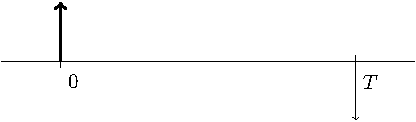
\includegraphics[width=1\linewidth]{three_files/figure-latex/unnamed-chunk-3-1} \end{center}

\begin{enumerate}
\def\labelenumi{(\alph{enumi})}
\setcounter{enumi}{1}
\tightlist
\item
\end{enumerate}

\begin{center}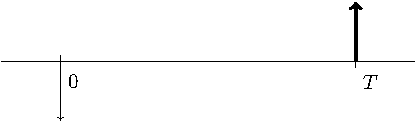
\includegraphics[width=0.8\linewidth]{three_files/figure-latex/unnamed-chunk-4-1} \end{center}

\begin{enumerate}
\def\labelenumi{(\alph{enumi})}
\setcounter{enumi}{2}
\tightlist
\item
\end{enumerate}

\begin{center}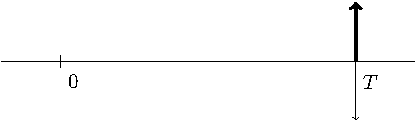
\includegraphics[width=0.8\linewidth]{three_files/figure-latex/unnamed-chunk-5-1} \end{center}

\begin{enumerate}
\def\labelenumi{(\alph{enumi})}
\setcounter{enumi}{3}
\tightlist
\item
\end{enumerate}

\begin{center}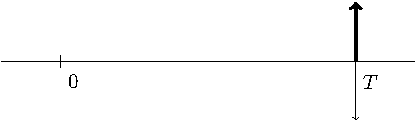
\includegraphics[width=0.8\linewidth]{three_files/figure-latex/unnamed-chunk-6-1} \end{center}

하나씩 살펴보겠습니다.

a는 우리가 일상적으로 생각하는 거래입니다. 1000을 pay하고, apple을 receive합니다.

b는현재 시점 \(t=0\)에 apple을 recieve하고, 미래의 특정 시점 \(t=T\)에 일정금액을 pay합니다. 이러한 거래는 신용을 기반으로 하는 거래로, 은행의 대출, 또는 채권(bond)이라는 금융상품과 관련이 있습니다.

\begin{example}[<U+C2E0><U+C6A9><U+C744> <U+AE30><U+BC18><U+C73C><U+B85C> <U+D55C> <U+AC70><U+B798>, credit transaction, debt security<U+C640> <U+AD00><U+B828><U+C774> <U+C788><U+C74C>]
\protect\hypertarget{exm:unnamed-chunk-7}{}{\label{exm:unnamed-chunk-7} \iffalse (\textless U+C2E0\textgreater\textless U+C6A9\textgreater\textless U+C744\textgreater{} \textless U+AE30\textgreater\textless U+BC18\textgreater\textless U+C73C\textgreater\textless U+B85C\textgreater{} \textless U+D55C\textgreater{} \textless U+AC70\textgreater\textless U+B798\textgreater, credit transaction, debt security\textless U+C640\textgreater{} \textless U+AD00\textgreater\textless U+B828\textgreater\textless U+C774\textgreater{} \textless U+C788\textgreater\textless U+C74C\textgreater) \fi{} }

b와 같은 형태의 거래를 예를 들어 보면,

\begin{enumerate}
\def\labelenumi{\arabic{enumi}.}
\item
  은행에서 1개월 만기 대출을 받아 apple을 사고, 1개월 후에 원금과 이자를 갚는다.
\item
  1개월 만기 채권을 발행하여, 채권가격 1000으로 현재시점에서 apple을 사고, 1개월 후 채권의 소유자에게 채권의 원금이 1000과 정하여진 coupon (채권 발행시 미리 정한 이자를 의미함)을 지불한다.
\item
  신용카드를 이용하여 apple을 사고, 1개월 후 신용카드 대금을 갚는다.
\end{enumerate}
\end{example}

\begin{example}[equity security]
\protect\hypertarget{exm:unnamed-chunk-8}{}{\label{exm:unnamed-chunk-8} \iffalse (equity security) \fi{} }

c는 주식이라는 금융상품의 초기 형태로 이해할 수 있습니다. 주식의 시작은 네덜란드 동인도 회사가 투자자금의 소유권에 대한 증서를 발행하는 것으로부터 시작되었습니다.
\end{example}

\hypertarget{uxac00uxc9c0uxc758-uxc11cuxb85c-uxb2e4uxb978-uxc0c1uxd488}{%
\section{3가지의 서로 다른 상품}\label{uxac00uxc9c0uxc758-uxc11cuxb85c-uxb2e4uxb978-uxc0c1uxd488}}

\begin{enumerate}
\def\labelenumi{(\alph{enumi})}
\setcounter{enumi}{3}
\tightlist
\item
\end{enumerate}

\begin{center}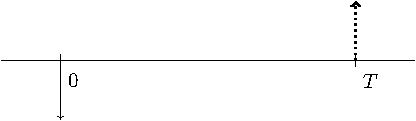
\includegraphics[width=0.8\linewidth]{three_files/figure-latex/unnamed-chunk-9-1} \end{center}

\begin{enumerate}
\def\labelenumi{(\alph{enumi})}
\setcounter{enumi}{4}
\tightlist
\item
\end{enumerate}

\begin{center}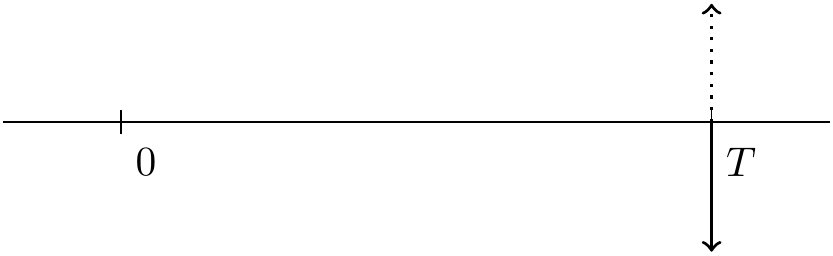
\includegraphics[width=0.8\linewidth]{three_files/figure-latex/unnamed-chunk-10-1} \end{center}

\begin{enumerate}
\def\labelenumi{(\alph{enumi})}
\setcounter{enumi}{5}
\tightlist
\item
\end{enumerate}

\begin{center}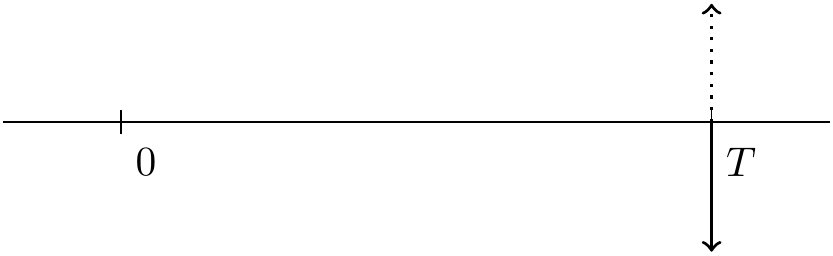
\includegraphics[width=0.8\linewidth]{three_files/figure-latex/unnamed-chunk-11-1} \end{center}

\hypertarget{part-financial-mathematics}{%
\part{Financial Mathematics}\label{part-financial-mathematics}}

\hypertarget{browian-motion}{%
\chapter{Browian Motion}\label{browian-motion}}

\hypertarget{part-advanced-finacial-engineering}{%
\part{Advanced Finacial Engineering}\label{part-advanced-finacial-engineering}}

\hypertarget{barrier-options}{%
\chapter{Barrier Options}\label{barrier-options}}

\hypertarget{part-tensorflow}{%
\part{TensorFlow}\label{part-tensorflow}}

\hypertarget{the-simplest-neural-network-ever}{%
\chapter{The Simplest Neural Network Ever}\label{the-simplest-neural-network-ever}}

\hypertarget{appendix-appendix}{%
\appendix}


\hypertarget{python}{%
\chapter{Python}\label{python}}

\hypertarget{linear-algebra}{%
\chapter{Linear Algebra}\label{linear-algebra}}

\hypertarget{calculus}{%
\chapter{Calculus}\label{calculus}}

\hypertarget{statistics}{%
\chapter{Statistics}\label{statistics}}

\end{document}
